% Provenance (never printed): see sources/outline_sources.md (Year 1:
% the Solar System, planetology). Kepler's laws, the moment of inertia and
% the Stefan--Boltzmann law are owned by the physics series and recalled
% here; the equilibrium temperature and the Bond albedo are re-founded from
% Book 2 grade 10. Curves computed in figdata/bachelor-1/planet_table.py;
% numbers of the exercises and problem in the Book 3 scratch calculator
% ch03.py.
\chapter{Planétologie comparée}\label{ch:b1:comparative-planetology}

Vénus et la Terre sont presque jumelles~: Vénus a \qty{95}{\percent} du rayon de
la Terre et \qty{81}{\percent} de sa masse. Pourtant la Terre a des océans, une
atmosphère d'azote et d'oxygène et des plaques mobiles, tandis que Vénus cache
sous ses nuages une surface à \qty{737}{K}, plus chaude que n'importe quel four
de cuisine, écrasée par une atmosphère de dioxyde de carbone à \qty{92}{bar}.
Mars, deux fois plus petite que la Terre, a une atmosphère mince et froide, des
volcans et des canyons géants, mais pas de plaques mobiles. Plus loin, Jupiter
et Saturne sont faites surtout d'hydrogène et d'hélium~; Uranus et Neptune,
surtout des glaces d'eau, de méthane et d'ammoniac. Comparer les planètes est le
seul moyen de mettre à l'épreuve ce que nous croyons savoir de la Terre~:
pourquoi son intérieur est en couches, pourquoi son climat est doux, pourquoi
elle seule a une tectonique des plaques. Ce chapitre pèse et mesure les
planètes, lit leur intérieur dans leur masse volumique et dans la répartition de
leur masse, compare leurs températures et leurs atmosphères, et s'achève sur
les satellites et les petits corps qui gardent la mémoire de la jeunesse du
Système solaire.
% ledger: nasa:venus, earth:Rmean, earth:mass, nasa:uranus-structure

\begin{recall}
Les planètes tournent autour du Soleil sur des ellipses, et le carré de la
période d'un satellite est proportionnel au cube de son demi-grand axe
(troisième loi de Kepler, dans le volume de physique de première année, où le
moment d'inertie d'un solide est aussi défini~; une sphère homogène a
$I = \tfrac25MR^2$). Un corps noir rayonne $\sigma T^4$ par unité de surface
(deuxième année). Le Système solaire et ses \omterm{def:b1:comparative-planetology:planet-types}{planètes telluriques} et géantes ont
été décrits au livre~1 (année~6)~; l'albédo et la \omterm{def:b1:comparative-planetology:equilibrium-temperature}{température d'équilibre} d'une
planète ont été rencontrés au livre~2 (année~10), et l'effet de serre au
livre~1 (année~9).
\end{recall}

\begin{omfigure}
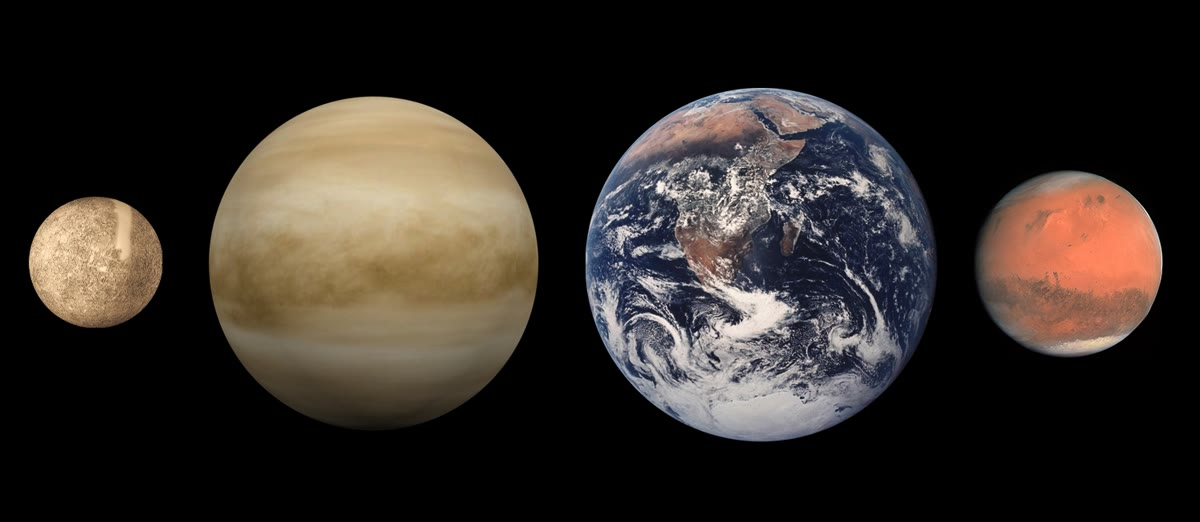
\includegraphics[width=0.85\linewidth]{images/book3/b1-terrestrial-planet-sizes.jpg}

{\small Les quatre \omterm{def:b1:comparative-planetology:planet-types}{planètes telluriques} à l'échelle, de gauche à droite
Mercure, Vénus, la Terre et Mars (distances hors échelle~; Vénus vue en lumière
visible, sa surface cachée sous les nuages). NASA, domaine public.}
% ledger: commons:terrestrial-sizes
\end{omfigure}

\section{Peser et mesurer les planètes}

Le rayon d'une planète se mesure à partir de son diamètre angulaire et de sa
distance ou, pour une planète visitée par des sondes, par altimétrie radar et
laser. Sa masse est plus difficile à obtenir~: on ne la perçoit que par la
gravité que la planète exerce sur autre chose.

\begin{method}[Masse d'une planète d'après l'orbite d'un satellite]\label{met:b1:comparative-planetology:mass}
Pour un satellite de masse négligeable sur une orbite presque circulaire de
rayon (demi-grand axe) $a$ et de période sidérale $T$ autour d'une planète de
masse $M$~:
\begin{enumerate}
  \item convertir $a$ en mètres et $T$ en secondes~;
  \item la troisième loi de Kepler donne $GM = 4\pi^2a^3/T^2$~: ce produit est ce
        que mesure l'orbite, et avec bien plus de précision que $G$ lui-même~;
  \item diviser par $G = \qty{6.6743e-11}{m^3.kg^{-1}.s^{-2}}$ pour obtenir $M$.
\end{enumerate}
Une planète sans satellite (Mercure, Vénus) se pèse de la même façon d'après
l'orbite, ou la déviation, d'une sonde qui passe à proximité.
\end{method}

\begin{example}
Io, le plus interne des grands satellites de Jupiter, orbite à
$a = \qty{421.8e3}{km}$ en \num{1.769138} jours, soit $T = \qty{152854}{s}$.
Alors
\[
  GM = \frac{4\pi^2\times(\qty{4.218e8}{m})^3}{(\qty{152854}{s})^2}
  = \qty{1.268e17}{m^3.s^{-2}}, \qquad
  M = \frac{\num{1.268e17}}{\num{6.6743e-11}} = \qty{1.900e27}{kg},
\]
ce qui s'accorde avec la masse tabulée de Jupiter, \qty{1.898e27}{kg}, à
\qty{0.1}{\percent} près. La masse propre d'Io, \num{4.7e-5} de celle de
Jupiter, est négligeable~; le petit excès vient du renflement équatorial de
Jupiter, qui attire un satellite proche un peu plus fort qu'une sphère de même
masse.
% ledger: nasa:io, nasa:jupiter, const:G
\end{example}

Avec la masse et le rayon vient la masse volumique moyenne $\bar\rho =
3M/(4\pi R^3)$, premier indice de ce dont est faite une planète. Les masses
volumiques des planètes se répartissent en deux groupes (voir la figure
ci-dessous)~: Mercure, Vénus, la Terre et Mars se situent entre environ
\num{3900} et \qty{5500}{kg.m^{-3}}, plus denses que n'importe quelle roche
courante~; les quatre planètes externes se situent entre \num{690} et
\qty{1640}{kg.m^{-3}}, près de la masse volumique de l'eau, celle de Saturne
étant même inférieure.
% ledger: planet:Mercury.density, planet:Mars.density, planet:Earth.density, planet:Saturn.density, planet:Neptune.density

\begin{omfigure}
\begin{tikzpicture}
\begin{axis}[omrecord, width=0.86\linewidth, height=6.2cm, xmode=log,
  xmin=800, xmax=150000, ymin=0, ymax=6300, xlabel={rayon équatorial (km)},
  ylabel={masse volumique moyenne (\unit{kg.m^{-3}})}, tick label style={font=\scriptsize},
  label style={font=\small}]
\addplot[only marks, mark=*, mark size=2.4pt, brown!70!black] table[x=R_km, y=density,
  restrict expr to domain={\thisrow{idx}}{0:2}] {figdata/out/bachelor-1-planet_table-bodies.dat};
\addplot[only marks, mark=*, mark size=2.4pt, brown!70!black] table[x=R_km, y=density,
  restrict expr to domain={\thisrow{idx}}{4:4}] {figdata/out/bachelor-1-planet_table-bodies.dat};
\addplot[only marks, mark=*, mark size=2.4pt, orange!85!black] table[x=R_km, y=density,
  restrict expr to domain={\thisrow{idx}}{5:6}] {figdata/out/bachelor-1-planet_table-bodies.dat};
\addplot[only marks, mark=*, mark size=2.4pt, omDef] table[x=R_km, y=density,
  restrict expr to domain={\thisrow{idx}}{7:8}] {figdata/out/bachelor-1-planet_table-bodies.dat};
\addplot[only marks, mark=o, mark size=2.4pt, black!60] table[x=R_km, y=density,
  restrict expr to domain={\thisrow{idx}}{3:3}] {figdata/out/bachelor-1-planet_table-bodies.dat};
\addplot[only marks, mark=o, mark size=2.4pt, black!60] table[x=R_km, y=density,
  restrict expr to domain={\thisrow{idx}}{9:9}] {figdata/out/bachelor-1-planet_table-bodies.dat};
\addplot[black!40, densely dashed] coordinates {(800,1000) (150000,1000)};
\begin{scope}[font=\scriptsize]
\node[left] at (axis cs:2439.5,5429) {Mercure};
\node[below left] at (axis cs:6052,5243) {Vénus};
\node[above] at (axis cs:6378,5514) {Terre};
\node[left] at (axis cs:3396,3934) {Mars};
\node[left] at (axis cs:1737.5,3340) {Lune};
\node[right] at (axis cs:1188,1850) {Pluton};
\node[above] at (axis cs:71492,1326) {Jupiter};
\node[left] at (axis cs:60268,687) {Saturne};
\node[right] at (axis cs:25559,1270) {Uranus};
\node[above] at (axis cs:24764,1638) {Neptune};
\node[above left, black!60] at (axis cs:150000,1000) {eau};
\end{scope}
\end{axis}
\end{tikzpicture}

{\small Masse volumique moyenne en fonction du rayon (échelle logarithmique)
pour les huit planètes (pleins~: telluriques, \omterm{def:b1:comparative-planetology:planet-types}{géantes gazeuses}, \omterm{def:b1:comparative-planetology:planet-types}{géantes de
glaces}), la Lune et Pluton (cercles ouverts). Données de la fiche planétaire de
la NASA.}
% ledger: planet:Mercury.diameter, planet:Venus.diameter, planet:Earth.diameter, planet:Moon.diameter, planet:Mars.diameter, planet:Jupiter.diameter, planet:Saturn.diameter, planet:Uranus.diameter, planet:Neptune.diameter, planet:Pluto.diameter, planet:Mercury.density, planet:Venus.density, planet:Earth.density, planet:Moon.density, planet:Mars.density, planet:Jupiter.density, planet:Saturn.density, planet:Uranus.density, planet:Neptune.density, planet:Pluto.density
\end{omfigure}

La masse volumique moyenne seule ne peut distinguer une planète faite d'un seul
matériau dense d'une planète dotée d'un centre très dense et d'une enveloppe
plus légère. Un second nombre le permet~: la façon dont la masse est répartie
entre le centre et la surface.

\begin{definition}[Facteur de moment d'inertie]\label{def:b1:comparative-planetology:moi}
Le \emph{facteur de moment d'inertie}\index{facteur de moment d'inertie} d'une
planète est le nombre
\[
  C = \frac{I}{MR^2} ,
\]
où $I$ est son moment d'inertie par rapport à son axe de rotation, $M$ sa masse
et $R$ son rayon moyen. Une sphère homogène a $C = \tfrac25 = 0.4$~; une planète
dont la masse volumique croît vers le centre a $C < 0.4$, d'autant plus petit
que la masse est plus concentrée.
\end{definition}

Le moment d'inertie se mesure à partir de la lente précession de l'axe de
rotation sous l'attraction du Soleil, avec l'aplatissement du champ de gravité
de la planète. Les valeurs sont parlantes~: la Lune, $C = 0.394$, est presque
homogène~; Mars, $0.366$, et la Terre, $0.3308$, sont nettement différenciées en
couches~; Jupiter, $0.254$, et Saturne, $0.210$, ont la plus grande partie de
leur masse rassemblée vers leur centre.
% ledger: nasa:moon, nasa:mars, earth:MoI, nasa:jupiter, nasa:saturn

\section{De quoi sont faites les planètes}

\begin{definition}[Planètes telluriques et planètes géantes]\label{def:b1:comparative-planetology:planet-types}
Une \emph{planète tellurique}\index{planete tellurique@planète tellurique} est une planète faite surtout de roche
silicatée et de fer, avec une surface solide~: Mercure, Vénus, la Terre et
Mars. Une \emph{planète géante}\index{planete geante@planète géante} est une planète de masse plusieurs fois
supérieure à celle de la Terre, faite surtout d'éléments légers et de leurs
composés et dépourvue de surface solide. Une \emph{géante gazeuse}\index{geante gazeuse@géante gazeuse}
est une planète géante faite surtout d'hydrogène et d'hélium~: Jupiter et
Saturne. Une \emph{géante de glaces}\index{geante de glaces@géante de glaces} est une planète géante faite surtout
des composés que les astronomes appellent glaces --- eau, méthane et ammoniac
--- sous une enveloppe d'hydrogène et d'hélium~: Uranus et Neptune.
\end{definition}

Les atmosphères que mesurent les sondes et les télescopes confirment cette
division. Celle de Jupiter est faite de \qty{89.8}{\percent} d'hydrogène et de
\qty{10.2}{\percent} d'hélium en volume, celle de Saturne de
\qty{96.3}{\percent} et \qty{3.25}{\percent}~; pour Uranus, au moins
\qty{80}{\percent} de la masse est un fluide chaud et dense d'eau, de méthane
et d'ammoniac au-dessus d'un petit noyau rocheux. La masse volumique moyenne
d'une \omterm{def:b1:comparative-planetology:planet-types}{géante gazeuse} reste faible bien que son centre soit fortement comprimé,
parce que l'hydrogène est l'élément le plus léger~; une \omterm{def:b1:comparative-planetology:planet-types}{géante de glaces} est
plus dense que Saturne parce que ses glaces sont plus lourdes que l'hydrogène.
% ledger: nasa:jupiter, nasa:saturn, nasa:uranus-structure

Les \omterm{def:b1:comparative-planetology:planet-types}{planètes telluriques} sont en couches comme la Terre~: un noyau riche en fer
sous un manteau silicaté et une croûte mince. Le modèle le plus simple qui
utilise les deux nombres mesurés, la masse volumique moyenne et le \omterm{def:b1:comparative-planetology:moi}{facteur de
moment d'inertie}, a deux couches.

\begin{proposition}[La planète à deux couches]\label{prop:b1:comparative-planetology:two-layer}
Modélisons une planète de rayon $R$ par un noyau de rayon $xR$ et de masse
volumique uniforme $\rho_c$ à l'intérieur d'un manteau de masse volumique
uniforme $\rho_m$. Sa masse volumique moyenne et son \omterm{def:b1:comparative-planetology:moi}{facteur de moment
d'inertie} sont
\[
  \bar\rho = \rho_m + (\rho_c - \rho_m)\,x^3 , \qquad
  C = \frac25\,\frac{\rho_m + (\rho_c - \rho_m)\,x^5}{\bar\rho} .
\]
Connaissant $\bar\rho$, $C$ et une masse volumique supposée du manteau $\rho_m$,
le rayon relatif du noyau s'en déduit~:
\[
  x^2 = \frac{\tfrac52C\bar\rho - \rho_m}{\bar\rho - \rho_m} ,
  \qquad \rho_c = \rho_m + \frac{\bar\rho - \rho_m}{x^3} .
\]
\end{proposition}

\begin{proof}
La planète est une sphère homogène de masse volumique $\rho_m$ et de rayon $R$
plus une sphère de rayon $xR$ de masse volumique en excès $\rho_c - \rho_m$. Les
masses s'ajoutent~:
$M = \tfrac43\pi R^3[\rho_m + (\rho_c - \rho_m)x^3]$, et la division par le
volume donne $\bar\rho$. Les moments d'inertie par rapport au même axe
s'ajoutent aussi~; une sphère homogène de masse volumique $\rho$ et de rayon $r$
a
$I = \tfrac25\cdot\tfrac43\pi\rho r^3\cdot r^2 = \tfrac{8\pi}{15}\rho r^5$,
donc $I = \tfrac{8\pi}{15}R^5[\rho_m + (\rho_c - \rho_m)x^5]$. La division par
$MR^2 = \tfrac43\pi\bar\rho R^5$ donne $C$. Enfin les deux équations s'écrivent
$(\rho_c - \rho_m)x^3 = \bar\rho - \rho_m$ et $(\rho_c - \rho_m)x^5 =
\tfrac52C\bar\rho - \rho_m$~; la division de la seconde par la première donne
$x^2$, et la première donne $\rho_c$.
\end{proof}

Le modèle a trois inconnues pour deux données, donc l'une d'elles, la masse
volumique du manteau, doit être supposée d'après ce que pèsent, sous pression,
des roches de composition convenable. La réponse est sensible à ce choix quand
$C$ est proche de $0.4$, car $\tfrac52C\bar\rho - \rho_m$ est alors une petite
différence de grands nombres (\cref{exo:b1:comparative-planetology:10} et le
problème). Le modèle ignore aussi la compression du manteau par son propre
poids, qui, dans une planète aussi grande que la Terre, élève la masse
volumique du manteau profond bien au-dessus de celle des roches de surface~;
pour la Terre, la sismologie fait bien mieux (\cref{ch:b1:layered-earth}). Des
sismomètres posés sur Mars ont maintenant fait de même pour cette planète~: là
où le tableau planétaire donne un rayon du noyau de \qty{1830}{km}, les
résultats récents n'indiquent que \qty{1650}{km} à \qty{1675}{km}.
% ledger: nasa:mars-core

\begin{omfigure}
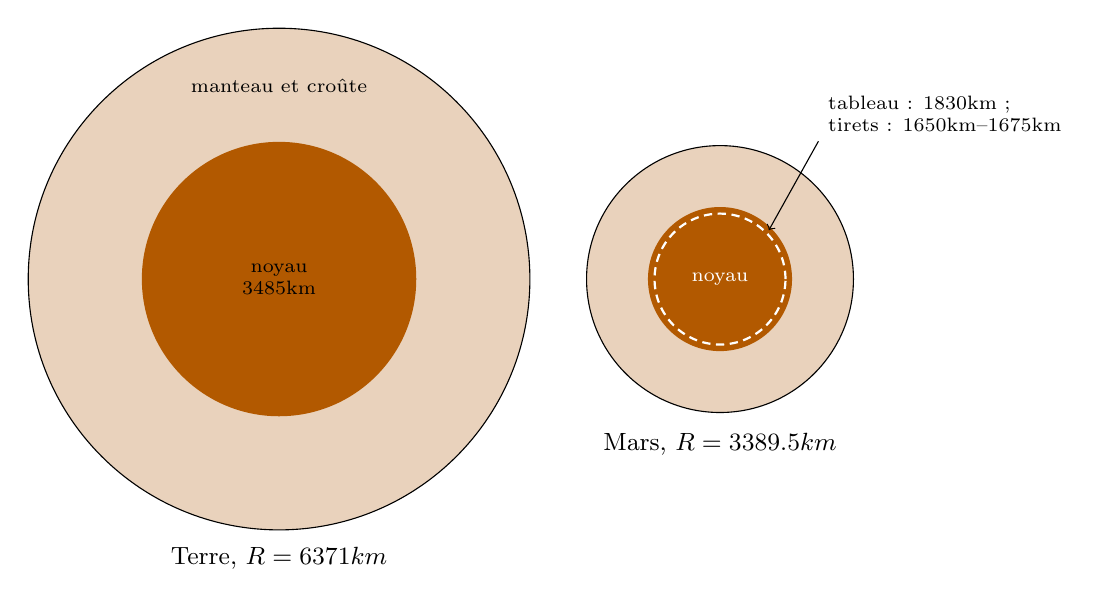
\begin{tikzpicture}[font=\scriptsize]
% scale: 0.5 cm per 1000 km
\fill[brown!35] (0,0) circle (3.1855cm);
\fill[orange!70!black] (0,0) circle (1.7425cm);
\draw (0,0) circle (3.1855cm);
\node[align=center] at (0,0) {noyau\\ \qty{3485}{km}};
\node[align=center] at (0,2.45) {manteau et croûte};
\node at (0,-3.55) {\small Terre, $R = \qty{6371}{km}$};
\begin{scope}[xshift=5.6cm]
\fill[brown!35] (0,0) circle (1.6948cm);
\fill[orange!70!black] (0,0) circle (0.915cm);
\draw[white, densely dashed, thick] (0,0) circle (0.8313cm);
\draw (0,0) circle (1.6948cm);
\node[align=center, white] at (0,0) {noyau};
\node at (0,-2.1) {\small Mars, $R = \qty{3389.5}{km}$};
\draw[->] (1.25,1.75) node[above right, align=left] {tableau~: \qty{1830}{km}~;\\ tirets~: \qty{1650}{km}--\qty{1675}{km}} -- (0.62,0.62);
\end{scope}
\end{tikzpicture}

{\small La Terre et Mars à l'échelle, avec leurs noyaux. Pour Mars, le trait
plein est le rayon du noyau du tableau planétaire et le cercle en tirets le
rayon plus petit indiqué par les résultats sismiques récents. Les deux noyaux
sont riches en fer~; celui de la Terre a une partie interne solide, non
dessinée.}
% ledger: earth:Rmean, earth:Rcore, nasa:mars, nasa:mars-core
\end{omfigure}

\section{Atmosphères et surfaces}

La température d'une planète est fixée d'abord par la lumière solaire qu'elle
absorbe. L'irradiance $S$ à sa distance $d$ du Soleil décroît en $1/d^2$
(\cref{prop:b1:observing-the-sky:inverse-square})~: \qty{1361}{W.m^{-2}} à
la Terre, \qty{2601}{W.m^{-2}} à Vénus, \qty{586}{W.m^{-2}} à Mars,
\qty{50}{W.m^{-2}} à Jupiter. Une partie en est directement renvoyée.
% ledger: earth:TSI, nasa:venus, nasa:mars, nasa:jupiter

\begin{definition}[Albédo de Bond]\label{def:b1:comparative-planetology:albedo}
L'\emph{albédo de Bond}\index{albedo de Bond@albédo de Bond} $A$ d'une planète est la fraction de la puissance totale
de la lumière solaire qui tombe sur elle qu'elle réfléchit et diffuse vers
l'espace, sur toutes les longueurs d'onde et dans toutes les directions.
\end{definition}

La neige fraîche et les nuages brillants réfléchissent beaucoup, la roche sombre
et la mer libre peu. Vénus, enveloppée de nuages brillants, a $A = 0.77$~; la
Terre $0.294$~; Mars $0.250$~; la Lune, roche gris sombre, $0.11$.
% ledger: nasa:venus, earth:albedo, nasa:mars, nasa:moon

\begin{definition}[Température d'équilibre]\label{def:b1:comparative-planetology:equilibrium-temperature}
La \emph{température d'équilibre}\index{temperature d'equilibre@température d'équilibre} $T_\mathrm{eq}$
d'une planète est la température uniforme à laquelle un corps noir de la taille
de la planète rayonnerait vers l'espace exactement la puissance que la planète
absorbe du Soleil.
\end{definition}

\begin{proposition}[Température d'équilibre]\label{prop:b1:comparative-planetology:teq}
Une planète d'\omterm{def:b1:comparative-planetology:albedo}{albédo de Bond} $A$ qui reçoit l'irradiance $S$ a
\[
  T_\mathrm{eq} = \left(\frac{S(1 - A)}{4\sigma}\right)^{1/4},
  \qquad \sigma = \qty{5.6704e-8}{W.m^{-2}.K^{-4}} .
\]
\end{proposition}

\begin{proof}
La planète intercepte la lumière solaire qui tombe sur sa section droite, un
disque d'aire $\pi R^2$, et en absorbe la fraction $1 - A$~: elle absorbe $S(1 - A)\pi
R^2$. Un corps noir (loi de Stefan--Boltzmann, admise du volume de physique de
deuxième année) à la température uniforme $T$ rayonne $\sigma T^4$ par mètre
carré de toute sa surface, $4\pi R^2$. En égalant les deux puissances,
$4\pi R^2\sigma T^4 = S(1 - A)\pi R^2$, et le facteur 4 est le rapport de l'aire
de la sphère à sa section droite.
\end{proof}

Avec les valeurs ci-dessus, $T_\mathrm{eq}$ vaut \qty{255}{K} pour la Terre,
\qty{227}{K} pour Vénus, \qty{210}{K} pour Mars et \qty{270}{K} pour la Lune.
Vénus, bien que plus proche du Soleil, sort plus froide que la Terre~: ses
nuages réfléchissent les trois quarts de la lumière solaire. La figure
ci-dessous place ces valeurs à côté des températures moyennes de surface
mesurées. Les écarts sont l'effet de serre, que les paragraphes suivants et les
chapitres sur le climat (\cref{ch:b1:radiation-heat-transport}) rendent
quantitatif~: environ \qty{33}{K} pour la Terre, environ \qty{510}{K} pour
Vénus, seulement environ \qty{4}{K} pour Mars.
% ledger: const:sigma, earth:Tsurf, nasa:venus, nasa:mars, planet:Moon.Tmean

\begin{omfigure}
\begin{tikzpicture}
\begin{axis}[ybar, bar width=12pt, width=0.72\linewidth, height=5.8cm,
  ymin=0, ymax=820, xmin=-0.6, xmax=3.6, xtick={0,1,2,3},
  xticklabels={Lune, Mars, Terre, Vénus}, ylabel={température (K)},
  tick label style={font=\scriptsize}, label style={font=\small},
  ymajorgrids, grid style={black!12}, axis lines*=left,
  legend style={font=\scriptsize, at={(0.03,0.97)}, anchor=north west, draw=none},
  nodes near coords, nodes near coords style={font=\tiny},
  every node near coord/.append style={/pgf/number format/fixed, /pgf/number format/precision=0}]
\addplot[fill=omDef!55, draw=omDef] table[x=idx, y=Teq] {figdata/out/bachelor-1-planet_table-temps.dat};
\addplot[fill=omThm!60, draw=omThm] table[x=idx, y=Tsurf] {figdata/out/bachelor-1-planet_table-temps.dat};
\legend{température d'équilibre, température moyenne de surface}
\end{axis}
\end{tikzpicture}

{\small \omterm{def:b1:comparative-planetology:equilibrium-temperature}{Température d'équilibre} (calculée à partir de l'irradiance et de
l'\omterm{def:b1:comparative-planetology:albedo}{albédo de Bond}) et température moyenne de surface mesurée de quatre corps.
L'atmosphère réchauffe la Terre et surtout Vénus~; la mince atmosphère de Mars
fait peu~; la Lune, sans atmosphère, est en moyenne plus froide que sa
\omterm{def:b1:comparative-planetology:equilibrium-temperature}{température d'équilibre}.}
% ledger: nasa:moon, nasa:mars, earth:TSI, earth:albedo, earth:Tsurf, nasa:venus, planet:Moon.Tmean, const:sigma
\end{omfigure}

La température moyenne de la Lune, environ \qty{253}{K}, est inférieure à sa
\omterm{def:b1:comparative-planetology:equilibrium-temperature}{température d'équilibre}. Ce n'est pas un paradoxe~: sans atmosphère ni océan
pour transporter la chaleur, la face éclairée est très chaude et la face
nocturne très froide, et comme l'émission croît en $T^4$, un corps aux
températures inégales rayonne la puissance absorbée avec une température
moyenne plus basse qu'un corps uniforme
(\cref{exo:b1:comparative-planetology:11}).

Une atmosphère fait deux choses~: elle laisse passer l'essentiel de la lumière
solaire et elle absorbe une partie de l'infrarouge émis par le sol, en en
réémettant une partie vers le bas. L'ampleur du réchauffement de la surface
dépend de la quantité de gaz absorbant au-dessus de chaque mètre carré. La
pression au sol mesure exactement cela~: $p = mg$ pour une colonne de masse $m$
par mètre carré. L'atmosphère de Vénus, à \qty{92}{bar}, est à
\qty{96.5}{\percent} du dioxyde de carbone~; celle de Mars, à seulement
\qty{6.36}{mbar} en moyenne, est elle aussi à \qty{95.1}{\percent} du dioxyde de
carbone, mais elle contient environ soixante fois moins de gaz au-dessus de
chaque mètre carré que celle de la Terre, et très peu de vapeur d'eau. Les deux
planètes ont une atmosphère de dioxyde de carbone~; une seule l'a épaisse.
% ledger: nasa:venus, nasa:mars, earth:psurf

\begin{omfigure}
\begin{minipage}{0.4\linewidth}
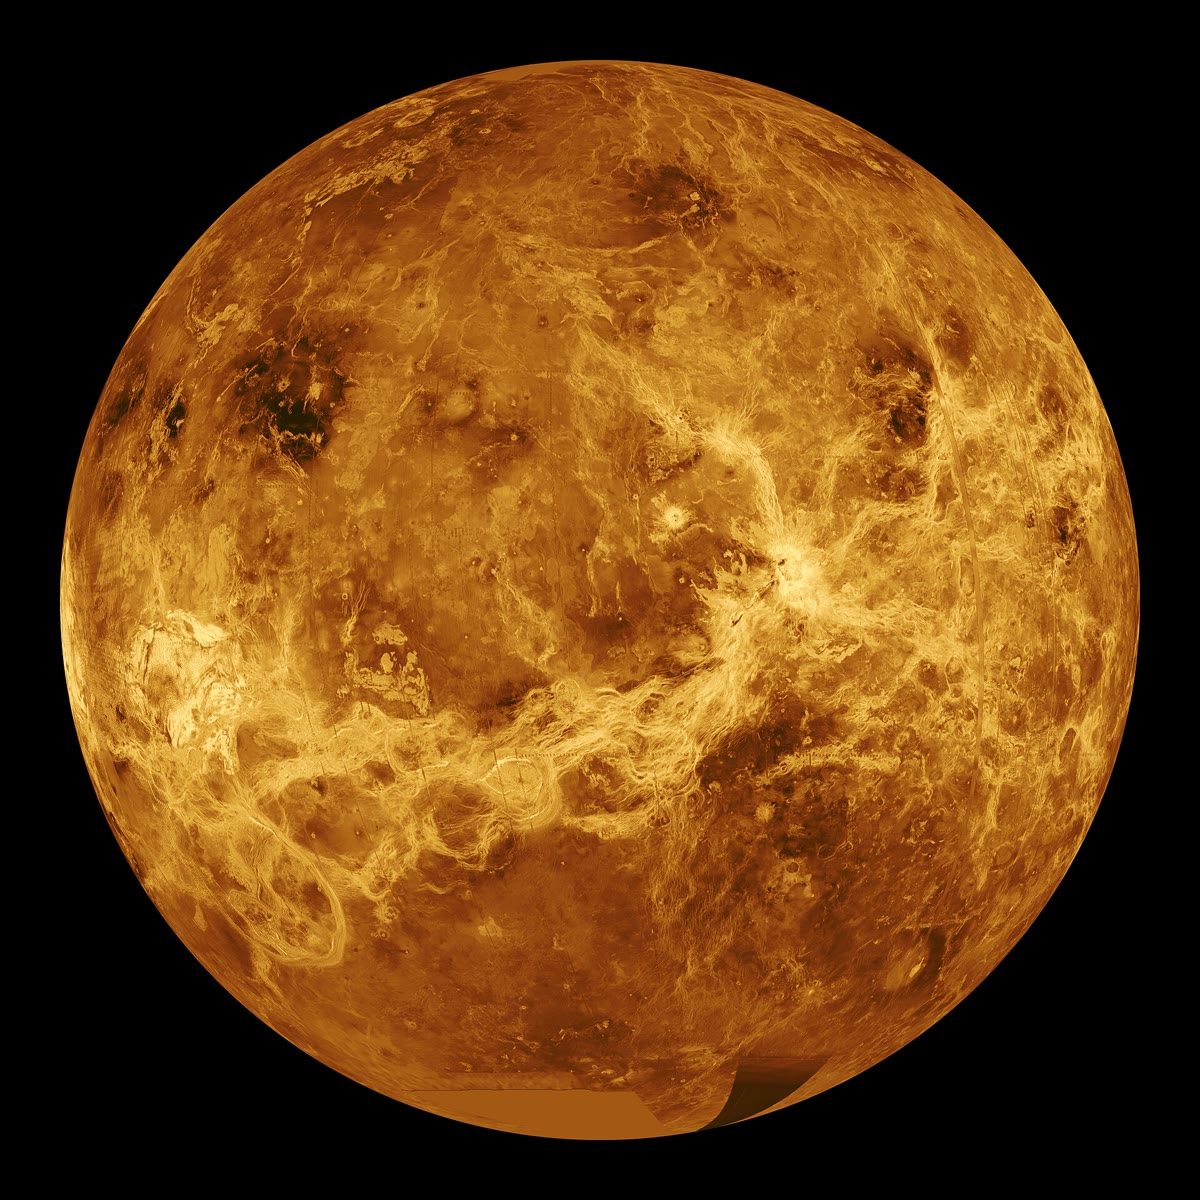
\includegraphics[width=\linewidth]{images/book3/b1-venus-radar-globe.jpg}
\end{minipage}\hspace{0.06\linewidth}
\begin{minipage}{0.4\linewidth}
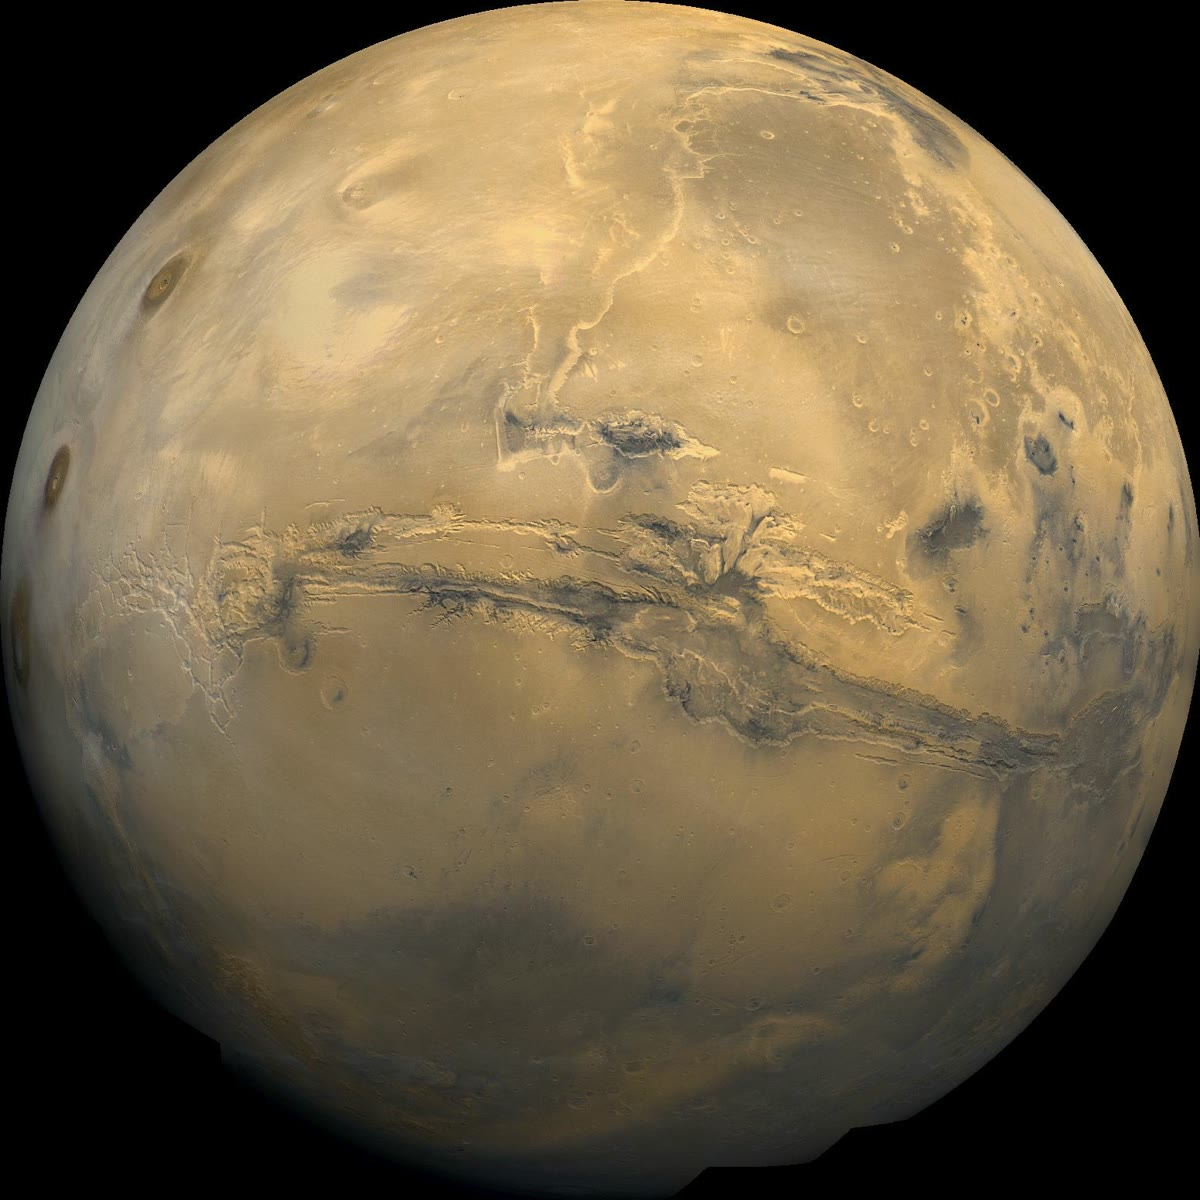
\includegraphics[width=\linewidth]{images/book3/b1-mars-valles-marineris.jpg}
\end{minipage}

{\small À gauche~: la surface de Vénus vue à travers ses nuages par le radar de
la sonde Magellan, projetée sur un globe simulé par ordinateur (les couleurs
sont simulées). À droite~: Mars vue de l'orbiteur Viking~1, mosaïque centrée sur
le système de canyons de Valles Marineris. NASA/JPL et NASA/USGS, domaine
public.}
% ledger: commons:venus-globe, commons:mars-valles
\end{omfigure}

Les surfaces portent le témoignage de ce qui les a façonnées. Les cratères
d'impact s'accumulent sur toute surface exposée à l'espace, si bien qu'une
surface fortement cratérisée, comme la plus grande partie de celle de la Lune ou
de Mercure, est ancienne, et qu'une surface peu cratérisée a été renouvelée~:
par des coulées de lave, par l'érosion, ou par les plaques qui ramènent le fond
océanique de la Terre dans le manteau. Des plaines volcaniques et des volcans se
trouvent sur toutes les \omterm{def:b1:comparative-planetology:planet-types}{planètes telluriques}. Des failles, des rifts et des
chaînes plissées montrent que les lithosphères de Vénus et de Mars ont été
déformées~; mais de toutes les planètes, seule la Terre montre aujourd'hui une
lithosphère brisée en plaques qui se déplacent comme des blocs rigides, avec des
dorsales là où elles se fabriquent et des fosses là où elles s'enfoncent.
Pourquoi la Terre seule a une tectonique des plaques fait encore débat~; la
présence d'eau, qui affaiblit les roches, est l'une des raisons avancées.

\section{Satellites et petits corps}

La Lune, dont le diamètre est le quart de celui de la Terre, est grande pour un
satellite. Sa masse volumique, \qty{3340}{kg.m^{-3}}, proche de celle des roches
du manteau terrestre, et son \omterm{def:b1:comparative-planetology:moi}{facteur de moment d'inertie}, proche de $0.4$,
montrent qu'elle n'a tout au plus qu'un petit noyau de fer. Les \omterm{def:b1:comparative-planetology:planet-types}{planètes
géantes} possèdent des systèmes de satellites qui sont des mondes à part entière
(voir les photographies ci-dessous). Io, le plus interne des quatre grands
satellites de Jupiter, est le monde le plus actif volcaniquement du Système
solaire, avec des centaines de volcans, chauffé par les marées que Jupiter y
soulève~; le volcanisme le remodèle plus vite que les impacts ne peuvent y
marquer de grands cratères. Europe, de masse volumique \qty{3010}{kg.m^{-3}},
est de la roche sous une croûte de glace, et de fortes présomptions indiquent un
océan salé sous cette croûte. Ganymède et Callisto, de masses volumiques
\num{1940} et \qty{1830}{kg.m^{-3}}, sont faits de roche et de glace en
proportions comparables.
Titan, le plus grand satellite de Saturne, est le seul satellite à atmosphère
dense, surtout d'azote avec un peu de méthane, et le seul monde, hormis la
Terre, qui ait des rivières, des lacs et des mers à sa surface --- de méthane et
d'éthane liquides~; il cache lui aussi probablement un océan d'eau.
% ledger: planet:Moon.diameter, planet:Earth.diameter, planet:Moon.density, nasa:moon, nasa:io-facts, nasa:europa, nasa:europa-facts, nasa:ganymede, nasa:titan-facts

\begin{omfigure}
\begin{minipage}{0.4\linewidth}
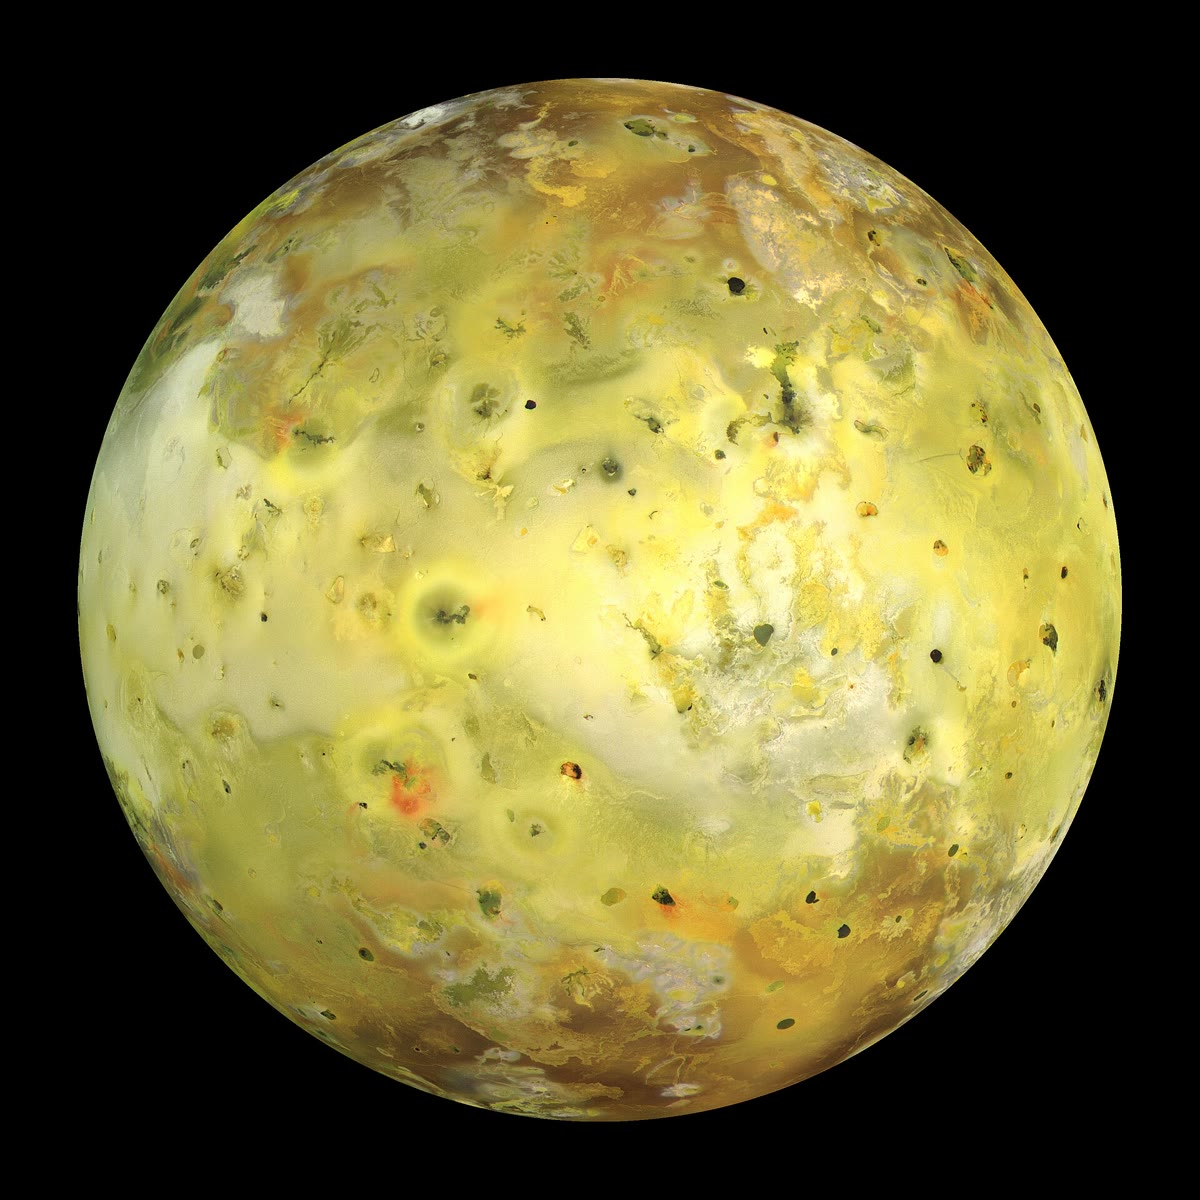
\includegraphics[width=\linewidth]{images/book3/b1-io.jpg}
\end{minipage}\hspace{0.06\linewidth}
\begin{minipage}{0.4\linewidth}
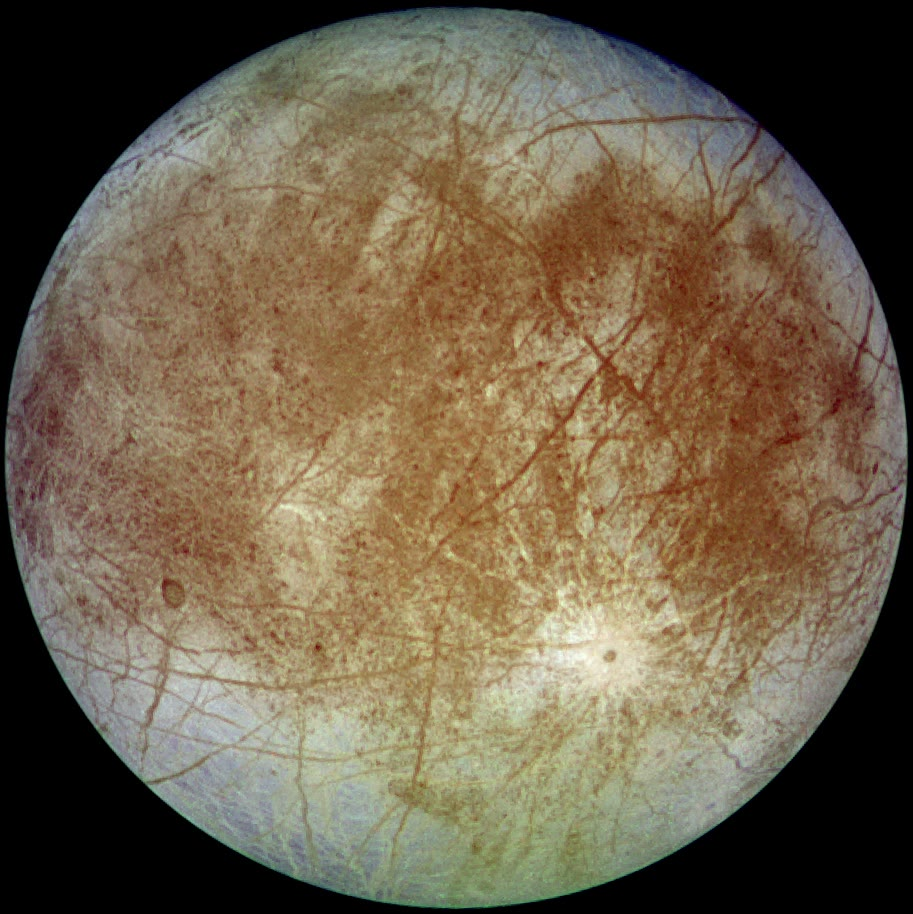
\includegraphics[width=\linewidth]{images/book3/b1-europa.jpg}
\end{minipage}

{\small Deux des grands satellites de Jupiter vus par la sonde Galileo. À
gauche~: Io, dont la surface est parsemée de centres volcaniques et colorée par
des composés soufrés et des laves. À droite~: Europe en couleurs naturelles
approchées~; les longues lignes sombres sont des fractures de sa croûte de
glace. NASA/JPL/University of Arizona et NASA/JPL/DLR, domaine public.}
% ledger: commons:io, commons:europa, nasa:io-facts, nasa:europa
\end{omfigure}

\begin{definition}[Astéroïde, comète, objet transneptunien]\label{def:b1:comparative-planetology:small-bodies}
Un \emph{astéroïde}\index{asteroide@astéroïde} est un petit corps rocheux ou métallique qui orbite autour du
Soleil, trop petit pour être une planète et dépourvu de l'enveloppe de gaz et de
poussière d'une comète~; la plupart orbitent entre Mars et Jupiter. Une
\emph{comète}\index{comete@comète} est un petit corps de glace et de poussière qui, lorsque son
orbite l'amène près du Soleil, libère du gaz et de la poussière formant autour
de lui une enveloppe lumineuse et des queues dirigées à l'opposé du Soleil. Un
\emph{objet transneptunien}\index{objet transneptunien} est un corps du Système
solaire dont l'orbite se situe, en moyenne, au-delà de celle de Neptune.
\end{definition}

Les \omterm{def:b1:comparative-planetology:small-bodies}{objets transneptuniens} de la ceinture de Kuiper, zone en forme de disque
au-delà de Neptune, sont des corps de glace et de roche laissés par la
formation des planètes~; Pluton, classée planète naine depuis 2006, en fait
partie. Les \omterm{def:b1:comparative-planetology:small-bodies}{astéroïdes} sont les débris d'une région où aucune planète ne s'est
formée. Des morceaux d'\omterm{def:b1:comparative-planetology:small-bodies}{astéroïdes}, et quelques-uns de la Lune et de Mars,
tombent sur la Terre sous forme de météorites. Ce sont les seuls échantillons
d'autres mondes que nous ayons en main, hormis ceux rapportés par des sondes, et
certains ont peu changé depuis la formation du Système solaire~; leurs classes,
et ce qu'elles disent de la composition de la Terre et de l'âge du Système
solaire, font l'objet du volume de deuxième année.
% ledger: nasa:pluto-facts

\section{Exercices}

\begin{exercise}[$\star$]\label{exo:b1:comparative-planetology:1}
Jupiter a une masse de \qty{1898.13e24}{kg} et un rayon moyen de
\qty{69911}{km}. Calculer sa masse volumique moyenne et la comparer à celle de
l'eau, \qty{1000}{kg.m^{-3}}.
\end{exercise}

\begin{exercise}[$\star$]\label{exo:b1:comparative-planetology:2}
À l'aide de la figure des masses volumiques et des rayons, classer Mercure,
Saturne, Uranus et Vénus parmi les \omterm{def:b1:comparative-planetology:planet-types}{planètes telluriques}, les \omterm{def:b1:comparative-planetology:planet-types}{géantes gazeuses} ou
les \omterm{def:b1:comparative-planetology:planet-types}{géantes de glaces}, et justifier chaque choix par le rayon et la masse
volumique.
\end{exercise}

\begin{exercise}[$\star$]\label{exo:b1:comparative-planetology:3}
Vénus reçoit \qty{2601.3}{W.m^{-2}} et a un \omterm{def:b1:comparative-planetology:albedo}{albédo de Bond} de 0.77. Calculer sa
\omterm{def:b1:comparative-planetology:equilibrium-temperature}{température d'équilibre}. Pourquoi est-elle inférieure à celle de la Terre, bien
que Vénus soit plus proche du Soleil~?
\end{exercise}

\begin{exercise}[$\star$]\label{exo:b1:comparative-planetology:4}
Classer la Lune ($C = 0.394$), Mars (0.366), la Terre (0.3308), Jupiter (0.254)
et Saturne (0.210) de la plus homogène à la plus concentrée en son centre. Que
vaudrait $C$ pour une planète dont toute la masse serait en un point en son
centre~?
\end{exercise}

\begin{exercise}[$\star\star$]\label{exo:b1:comparative-planetology:5}
Titan orbite autour de Saturne à $a = \qty{1221.87e3}{km}$ en \num{15.945421}
jours. Calculer la masse de Saturne et la comparer à la valeur tabulée
\qty{568.32e24}{kg}.
\end{exercise}

\begin{exercise}[$\star\star$]\label{exo:b1:comparative-planetology:6}
La Terre reçoit \qty{1361}{W.m^{-2}} à \qty{149.6e6}{km} du Soleil. Calculer
l'irradiance à Mars (\qty{228.0e6}{km}) et à Jupiter (\qty{778.5e6}{km}), et la
comparer aux valeurs tabulées \qty{586.2}{W.m^{-2}} et \qty{50.26}{W.m^{-2}}.
\end{exercise}

\begin{exercise}[$\star\star$]\label{exo:b1:comparative-planetology:7}
Montrer que, pour un albédo donné, $T_\mathrm{eq}$ varie comme $d^{-1/2}$.
Calculer $T_\mathrm{eq}$ pour Jupiter ($S = \qty{50.26}{W.m^{-2}}$, $A = 0.343$).
Si l'on trouvait que Jupiter rayonne plus de puissance qu'elle n'en absorbe du
Soleil, qu'est-ce que cela impliquerait pour son intérieur~?
\end{exercise}

\begin{exercise}[$\star\star$]\label{exo:b1:comparative-planetology:8}
Calculer le réchauffement par effet de serre $T_\mathrm{surf} - T_\mathrm{eq}$
de Vénus (\qty{737}{K}), de la Terre (\qty{288}{K}, $A = 0.294$) et de Mars
(\qty{214}{K}). Exprimer chacun comme fraction de $T_\mathrm{eq}$.
\end{exercise}

\begin{exercise}[$\star\star$]\label{exo:b1:comparative-planetology:9}
Pour une sphère homogène, montrer que $C = 0.4$ en intégrant les moments
d'inertie de fines coquilles sphériques (une coquille de rayon $r$ et de masse
$\mathrm dm$ a $\mathrm dI = \tfrac23 r^2\,\mathrm dm$). Quelle valeur a une
coquille creuse de rayon $R$~?
\end{exercise}

\begin{exercise}[$\star\star\star$]\label{exo:b1:comparative-planetology:10}
Mercure a $\bar\rho = \qty{5429}{kg.m^{-3}}$, $C = 0.35$ et un rayon de
\qty{2439.7}{km}. Avec une masse volumique du manteau de \qty{3300}{kg.m^{-3}},
utiliser le modèle à deux couches pour trouver son rayon du noyau, sa masse
volumique du noyau et la fraction de sa masse contenue dans le noyau. Qu'a de
remarquable Mercure~?
\end{exercise}

\begin{exercise}[$\star\star\star$]\label{exo:b1:comparative-planetology:11}
Modéliser un corps sans atmosphère dont l'hémisphère de jour est à la
température uniforme $T_1$ et l'hémisphère de nuit à $T_2$, rayonnant ensemble
la puissance absorbée. (a) Montrer que si $T_1^4 + T_2^4 = 2T_\mathrm{eq}^4$, la
température moyenne $(T_1 + T_2)/2$ est au plus égale à $T_\mathrm{eq}$, avec
égalité seulement lorsque $T_1 = T_2$. (b) Pour la Lune,
$T_\mathrm{eq} = \qty{270}{K}$~; prendre $T_2 = \qty{100}{K}$. Calculer $T_1$ et
la température moyenne.
\end{exercise}

\begin{exercise}[$\star\star\star$]\label{exo:b1:comparative-planetology:12}
Vénus a un rayon de \qty{6051.8}{km}, une pesanteur de surface de
\qty{8.9}{m.s^{-2}} et une pression au sol de \qty{92}{bar}. Calculer la masse
de son atmosphère, la comparer à celle de la Terre, \qty{5.1e18}{kg}, et à la
masse de Vénus, \qty{4.8673e24}{kg}. Que suggère cette comparaison sur l'endroit
où est stocké le dioxyde de carbone de la Terre~?
% ledger: earth:Matm, planet:Venus.gravity, nasa:venus
\end{exercise}

\section{Problème~: Peser et sonder Mars}

\begin{problem}[{Problème du week-end --- la masse de Mars d'après son satellite,
sa masse volumique et sa température, et la taille de son noyau}]
\label{pb:b1:comparative-planetology:1}
% ledger: nasa:phobos, nasa:mars, nasa:mars-core, const:G, const:sigma, earth:psurf, earth:gmean, planet:Mars.Prot, planet:Earth.density
% numbers computed in the scratch calculator calc/ch03.py from the rounded data
Phobos, le plus grand satellite de Mars, orbite à une distance moyenne de
\qty{9378}{km} du centre de Mars en \num{0.31891} jour. Mars a un rayon moyen de
\qty{3389.5}{km}, une période de rotation de \qty{24.6}{h}, un \omterm{def:b1:comparative-planetology:moi}{facteur de
moment d'inertie} $C = 0.366$, un \omterm{def:b1:comparative-planetology:albedo}{albédo de Bond} de 0.250 et une pression moyenne
au sol de \qty{6.36}{mbar}~; elle reçoit \qty{586.2}{W.m^{-2}} du Soleil, et sa
température moyenne de surface est d'environ \qty{214}{K}. Phobos a une masse de
\qty{1.06e16}{kg}. On prend $G = \qty{6.6743e-11}{m^3.kg^{-1}.s^{-2}}$
et $\sigma = \qty{5.6704e-8}{W.m^{-2}.K^{-4}}$.

\medskip
\noindent\textbf{Partie I --- Peser Mars.}
\begin{enumerate}
  \item Convertir la période de Phobos en secondes.
  \item Calculer $GM$ pour Mars.
  \item En déduire la masse de Mars.
  \item Est-il légitime de négliger la masse de Phobos~?
  \item Calculer la vitesse orbitale de Phobos.
  \item Comparer la période de Phobos à la rotation de Mars. Dans quel sens
        Phobos traverse-t-il le ciel de Mars~?
\end{enumerate}

\medskip
\noindent\textbf{Partie II --- Masse volumique et pesanteur.}
\begin{enumerate}[resume]
  \item Calculer le volume de Mars.
  \item Calculer sa masse volumique moyenne, arrondie à \qty{10}{kg.m^{-3}}.
  \item La comparer à celle de la Terre, \qty{5514}{kg.m^{-3}}. Donner deux
        raisons pour lesquelles la Terre est plus dense.
  \item Calculer la pesanteur à la surface de Mars.
  \item Calculer la vitesse de libération à la surface de Mars.
\end{enumerate}

\medskip
\noindent\textbf{Partie III --- Température et atmosphère.}
\begin{enumerate}[resume]
  \item Calculer la \omterm{def:b1:comparative-planetology:equilibrium-temperature}{température d'équilibre} de Mars.
  \item La comparer à la température moyenne de surface. Quelle est l'ampleur
        du réchauffement par effet de serre~?
  \item Calculer la masse de l'atmosphère au-dessus de chaque mètre carré de
        Mars, et la comparer à celle de la Terre ($p = \qty{1014}{hPa}$,
        $g = \qty{9.82}{m.s^{-2}}$).
  \item Calculer la masse totale de l'atmosphère de Mars.
  \item L'atmosphère de Mars est à \qty{95}{\percent} du dioxyde de carbone, et
        pourtant son réchauffement par effet de serre est faible. Proposer une
        explication.
\end{enumerate}

\medskip
\noindent\textbf{Partie IV --- Le noyau de Mars.}
\begin{enumerate}[resume]
  \item Que vaudrait $C$ si Mars était homogène~? Que dit la valeur mesurée~?
  \item Écrire la masse volumique moyenne d'une Mars à deux couches en fonction
        du rayon relatif du noyau $x$, de la masse volumique du manteau $\rho_m$
        et de la masse volumique du noyau $\rho_c$.
  \item Écrire son \omterm{def:b1:comparative-planetology:moi}{facteur de moment d'inertie} dans les mêmes termes.
  \item Montrer que $x^2 = (\tfrac52C\bar\rho - \rho_m)/(\bar\rho - \rho_m)$.
  \item Avec la masse volumique moyenne de la question 8 et $\rho_m =
        \qty{3500}{kg.m^{-3}}$, calculer $x$ et la masse volumique du noyau.
  \item Quelle fraction de la masse de Mars se trouve dans son noyau~?
  \item Recommencer la question 21 avec $\rho_m = 3450$ et
        \qty{3550}{kg.m^{-3}}. Que conclure sur la précision du modèle~?
  \item Donner le rayon du noyau de Mars d'après le modèle avec
        $\rho_m = \qty{3500}{kg.m^{-3}}$, et le comparer à la valeur du tableau
        planétaire, \qty{1830}{km}, et au résultat sismique récent,
        \qty{1650}{km} à \qty{1675}{km}.
\end{enumerate}
\end{problem}
